\chapter{DNA：通用遗传分子}\label{ch:g10:universal-dna}

在一间暗室中，蓝灯之下，两只白鼠中的一只
从鼻子到尾巴都发出绿光。它的每一个\omterm{def:g10:cells-common-unit:cell}{细胞}中
都带有一个\omterm{def:g10:universal-dna:gene}{基因}，取自一种在太平洋发光的水母——
而这只小鼠的\omterm{def:g10:cells-common-unit:cell}{细胞}读取这个水母\omterm{def:g10:universal-dna:gene}{基因}的方式，与水母自身的\omterm{def:g10:cells-common-unit:cell}{细胞}完全相同。
这个实验之所以能够成功，是因为所有生物都用同一种分子书写\omterm{def:g10:universal-dna:gene}{基因}，
使用同样的四种字母，并且按照同样的规则读取。
本章讨论的是这种分子，\omterm{def:g10:universal-dna:information}{DNA}：它如何构成，
其结构能解释什么，以及这只发光的小鼠证明了什么。

\section{遗传物质}

\begin{definition}[遗传信息]\label{def:g10:universal-dna:information}
\omterm{def:g10:cells-common-unit:cell}{细胞}的\emph{遗传信息}\index{遗传信息}是
一组指令，它从\omterm{def:g10:cells-common-unit:cell}{细胞}传递给其子\omterm{def:g10:cells-common-unit:cell}{细胞}，
也从亲代传递给子代，决定生物体的性状
以及其\omterm{def:g10:cells-common-unit:cell}{细胞}能够合成的\omterm{def:g10:chemistry-of-life:families}{蛋白质}。在所有生物中，它
由\emph{DNA}\index{DNA}（脱氧核糖\omterm{def:g10:chemistry-of-life:families}{核
酸}）分子携带，并与\omterm{def:g10:chemistry-of-life:families}{蛋白质}一起包装成\emph{染色体}\index{染色体}，
——存在于\omterm{def:g10:cells-common-unit:prokaryote}{真核细胞}的\omterm{def:g10:cells-common-unit:organelle}{细胞核}中，或游离于
细菌的\omterm{def:g10:cells-common-unit:cell}{细胞质}中。
\end{definition}

\begin{proposition}[DNA 是遗传分子]\label{prop:g10:universal-dna:material}
\omterm{def:g10:cells-common-unit:cell}{细胞}的遗传物质是它的 \omterm{def:g10:universal-dna:information}{DNA}，而不是其\omterm{def:g10:chemistry-of-life:families}{蛋白质}或任何
其他组分：把纯化的 \omterm{def:g10:universal-dna:information}{DNA} 从一种细菌菌株转移到另一种
细菌中，会使后者获得前一菌株的性状。
\end{proposition}
\begin{proof}[证据]
格里菲思（1928 年）发现，无害的肺炎细菌与
致死菌株被杀死的\omterm{def:g10:cells-common-unit:cell}{细胞}混合后，变得具有致死性，并且
此后各代都保持这一性状：死\omterm{def:g10:cells-common-unit:cell}{细胞}中的某种物质使它们发生了“转化”。
埃弗里、麦克劳德和麦卡蒂（1944 年）将死\omterm{def:g10:cells-common-unit:cell}{细胞}的提取物
分离为各类分子，并逐一检验：只有 \omterm{def:g10:universal-dna:information}{DNA}
组分能够引起转化；用能破坏 \omterm{def:g10:universal-dna:information}{DNA} 的酶处理提取物，转化效应消失，
而破坏\omterm{def:g10:chemistry-of-life:families}{蛋白质}的酶或
破坏 RNA 的酶则无影响。转化物质，因此也是
遗传性状的载体，就是 \omterm{def:g10:universal-dna:information}{DNA}。
\end{proof}

\begin{example}[DNA 的位置]\label{ex:g10:universal-dna:where}
一种对 \omterm{def:g10:universal-dna:information}{DNA} 具有特异性的染料可以使口腔上皮\omterm{def:g10:cells-common-unit:cell}{细胞}的\omterm{def:g10:cells-common-unit:organelle}{细胞核}着色，
\omterm{def:g10:cells-common-unit:cell}{细胞质}则不被染色；在分裂的\omterm{def:g10:cells-common-unit:cell}{细胞}中，它使紧缩的\omterm{def:g10:universal-dna:information}{染色体}着色。
细菌在一个没有膜包被的中央区域吸收这种染料。
在两者中，\omterm{def:g10:universal-dna:information}{DNA} 的量都会在每次分裂前加倍，
并在两个子\omterm{def:g10:cells-common-unit:cell}{细胞}之间平分——
这正是必须被复制和共享的信息所应有的表现。
\end{example}

\section{DNA 的结构}

\begin{definition}[核苷酸]\label{def:g10:universal-dna:nucleotide}
\omterm{def:g10:universal-dna:information}{DNA} 是由\emph{核苷酸}\index{核苷酸}连接成的链。每个
核苷酸由三部分构成：一个磷酸基团、一个糖
（脱氧核糖）和四种含氮
\emph{碱基}\index{碱基（DNA）}之一：腺嘌呤（A）、胸腺嘧啶（T）、鸟嘌呤（G）
和胞嘧啶（C）。糖与磷酸交替连接，构成链的
骨架；碱基则伸出骨架之外，每个核苷酸一个。
四种核苷酸的区别仅在于碱基，因此一条 \omterm{def:g10:universal-dna:information}{DNA} 链可以
用其碱基序列来描述，写成一串
字母：\texttt{ATGGCTTAC\dots}
\end{definition}

\begin{omfigure}
\begin{tikzpicture}[>=Stealth, font=\small]
  % left strand backbone
  \foreach \i in {0,...,5} {
    \draw[fill=gray!30] (0,{1.1*\i}) circle (0.22);           % phosphate
    \draw[fill=omDef!25] (0.9,{1.1*\i+0.15}) -- (1.35,{1.1*\i+0.45}) -- (1.35,{1.1*\i-0.15}) -- (0.9,{1.1*\i-0.45}) -- (0.55,{1.1*\i}) -- cycle; % sugar (pentagon)
    \draw (0.22,{1.1*\i}) -- (0.55,{1.1*\i});
    \draw (1.35,{1.1*\i+0.45}) -- (0,{1.1*\i+1.1-0.22});
  }
  \foreach \i in {0,...,5} {
    \draw[fill=gray!30] (7.6,{1.1*\i+0.55}) circle (0.22);
    \draw[fill=omDef!25] (6.7,{1.1*\i+0.55+0.15}) -- (6.25,{1.1*\i+0.55+0.45}) -- (6.25,{1.1*\i+0.55-0.15}) -- (6.7,{1.1*\i+0.55-0.45}) -- (7.05,{1.1*\i+0.55}) -- cycle;
    \draw (7.38,{1.1*\i+0.55}) -- (7.05,{1.1*\i+0.55});
  }
  \foreach \i in {0,...,4}
    \draw (6.25,{1.1*\i+0.55+0.45}) -- (7.6,{1.1*\i+0.55+1.1-0.22});
  % base pairs
  \foreach \i/\l/\r/\cl/\cr in {0/A/T/omThm/omMeth, 1/G/C/omProp/omDef,
      2/C/G/omDef/omProp, 3/T/A/omMeth/omThm, 4/A/T/omThm/omMeth, 5/G/C/omProp/omDef} {
    \draw[fill=\cl!40] (1.35,{1.1*\i+0.15-0.25}) rectangle (3.7,{1.1*\i+0.15+0.25});
    \node at (2.5,{1.1*\i+0.15}) {\l};
    \draw[fill=\cr!40] (3.9,{1.1*\i+0.15-0.25}) rectangle (6.25,{1.1*\i+0.15+0.25});
    \node at (5.1,{1.1*\i+0.15}) {\r};
    \draw[densely dotted, thick] (3.7,{1.1*\i+0.15}) -- (3.9,{1.1*\i+0.15});
  }
  \node[anchor=east, align=right] at (-0.4,2.9) {磷酸 \\ 与糖 \\ 骨架};
  \node[anchor=west, align=left] at (8.0,3.45) {第二条 \\ 链};
  \node[anchor=south] at (2.5,6.5) {成对的碱基};
  \draw[->] (0,-0.5) -- (0,-1.0) node[below] {链 1 的方向};
  \draw[->] (7.6,0.05) -- (7.6,-1.0) node[below] {链 2，方向相反};
  \draw[<->, thick] (8.9,0.15) -- (8.9,1.25) node[midway, right] {\qty{0.34}{nm}};
\end{tikzpicture}

{\small 图示为展开的两条 \omterm{def:g10:universal-dna:information}{DNA} 链。每条链都是由
\omterm{def:g10:universal-dna:nucleotide}{核苷酸}（磷酸、糖、碱基）构成的链。两条链的走向
方向相反，并通过碱基对结合在一起：A 总是与 T 相对，G
总是与 C 相对。相邻碱基对每隔 \qty{0.34}{nm} 出现一个。}
\end{omfigure}

\begin{proposition}[双螺旋]\label{prop:g10:universal-dna:helix}
一个 \omterm{def:g10:universal-dna:information}{DNA} 分子由两条链相互缠绕构成，形成
右手\emph{双螺旋}\index{双螺旋}结构，直径约为 \qty{2}{nm}，
每旋转一周含十个碱基对（\qty{3.4}{nm}）。两条链
走向相反，彼此以碱基相对，碱基
按照严格的
\emph{互补性}\index{互补性}规则配对：A 只与 T 配对，G
只与 C 配对。因此，一条链的序列决定了
另一条链的序列。
\end{proposition}
\begin{proof}[证据]
查加夫（1950 年）测定了多种物种的 \omterm{def:g10:universal-dna:information}{DNA} 碱基组成，
发现在每一种中，A 的含量都与 T 相等，G 的含量都与 C 相等，
而 A+T 与 G+C 的比例则因物种而异——这是一种配对
规则，而非化学上的偶然。富兰克林拍摄的 \omterm{def:g10:universal-dna:information}{DNA} 纤维
X 射线照片（1952 年）显示出直径为 \qty{2}{nm} 的螺旋结构特征，
螺距为 \qty{3.4}{nm}。沃森和克里克（1953 年）建立了唯一能同时符合上述两点的模型：
两条骨架位于外侧，成对的碱基位于内侧，A--T 与
G--C 碱基对宽度相同，因此螺旋结构是规则的。
\end{proof}

\begin{example}[数字中的查加夫规则]\label{ex:g10:universal-dna:chargaff}
人类 \omterm{def:g10:universal-dna:information}{DNA}：A 30.9\%，T 29.4\%，G 19.9\%，C 19.8\%——A$\,\approx\,$T
与 G$\,\approx\,$C 在测量精度内相等，且 A+T $= 60\%$。
\emph{E.~coli}：A 24.7\%，T 23.6\%，G 26.0\%，C 25.7\%，
A+T $= 48\%$。酵母：A+T $= 64\%$。若某 \omterm{def:g10:universal-dna:information}{DNA} 样品中 A 占 32\%，
由\omterm{prop:g10:universal-dna:helix}{互补性}可知，T 占 32\%，G 和 C 各占
$(100 - 64)/2 = 18\%$。
\end{example}

\begin{omfigure}
\begin{tikzpicture}
\begin{axis}[
  ybar, bar width=7pt,
  width=0.86\linewidth, height=5.4cm,
  axis x line=bottom, axis y line=left,
  ymin=0, ymax=40, ylabel={碱基含量（\%）}, ylabel style={font=\small},
  symbolic x coords={human, yeast, E. coli, wheat},
  xtick=data, xticklabels={人, 酵母, 大肠杆菌, 小麦}, tick label style={font=\small},
  enlarge x limits=0.18,
  legend style={at={(0.5,-0.2)}, anchor=north, legend columns=4,
                font=\small, draw=none},
]
\addplot[fill=omThm!50, draw=omThm] coordinates {(human,30.9) (yeast,31.3) (E. coli,24.7) (wheat,27.3)};
\addplot[fill=omMeth!60, draw=omMeth] coordinates {(human,29.4) (yeast,32.9) (E. coli,23.6) (wheat,27.1)};
\addplot[fill=omProp!50, draw=omProp] coordinates {(human,19.9) (yeast,18.7) (E. coli,26.0) (wheat,22.7)};
\addplot[fill=omDef!50, draw=omDef] coordinates {(human,19.8) (yeast,17.1) (E. coli,25.7) (wheat,22.8)};
\legend{A, T, G, C}
\end{axis}
\end{tikzpicture}

{\small 四个物种的 \omterm{def:g10:universal-dna:information}{DNA} 碱基组成。每个物种中，A 与 T 的柱高相符，
G 与 C 的柱高相符——这正是碱基配对的特征——
而 A+T 所占的比例因物种而异。}
\end{omfigure}

\begin{method}[写出互补链]\label{met:g10:universal-dna:complement}
已知一条链，在每个碱基下方写出其配对碱基（A$\leftrightarrow$T，
G$\leftrightarrow$C），然后以相反方向读出结果，
若练习的约定要求如此。对于
\texttt{5'-ATGGCTTAC-3'}，其配对链沿自身方向读取为
\texttt{5'-GTAAGCCAT-3'}。计数：一条含
$n_\mathrm{A}$ 个腺嘌呤的链与一条含 $n_\mathrm{A}$ 个胸腺嘧啶的链相对，
故整个分子中 $n_\mathrm{A} = n_\mathrm{T}$，且
$n_\mathrm{G} = n_\mathrm{C}$。
\end{method}

\begin{proposition}[结构所解释的内容]\label{prop:g10:universal-dna:explains}
由此结构可得遗传物质的两条性质。
 \begin{itemize}
  \item \emph{信息}：沿一条链的碱基顺序
        不受化学性质的限制，任何序列皆可能出现，
        因此序列可以携带信息，正如字母的排列承载文字。
        人类\omterm{def:g10:cells-common-unit:cell}{细胞}的每套\omterm{def:g10:universal-dna:information}{染色体}中含有 $\num{3.2e9}$ 个
        碱基对。
  \item \emph{复制}：由于每条链都决定另一条链，
        分子可以分开两条链，在每条链上合成新的配对链而被复制。
        该机制将在
        \cref{ch:g11:dna-replication}中讨论。
\end{itemize}
\end{proposition}
\admitted

\section{基因、等位基因、染色体}

\begin{definition}[基因与等位基因]\label{def:g10:universal-dna:gene}
一个\emph{基因}\index{基因}是 \omterm{def:g10:universal-dna:information}{DNA} 分子的一段——通常
包含数千个碱基对，其序列携带
制造一种\omterm{def:g10:chemistry-of-life:families}{蛋白质}（有时是一个有功能的 RNA 分子）的
指令。它在特定\omterm{def:g10:universal-dna:information}{染色体}上占据固定位置。
同一基因中仅相差若干碱基的各个版本，称为其
\emph{等位基因}\index{等位基因}：位置相同、功能相同、序列略有不同，
因此所编码的\omterm{def:g10:chemistry-of-life:families}{蛋白质}往往也略有不同。
\end{definition}

\begin{example}[数字举例]\label{ex:g10:universal-dna:numbers}
人类\omterm{def:g10:universal-dna:gene}{基因}组——即一整套\omterm{def:g10:universal-dna:information}{染色体}——含有
$\num{3.2e9}$ 个碱基对，约 $\num{20000}$ 个\omterm{def:g10:universal-dna:gene}{基因}；
它们仅占序列的百分之几。一个 \emph{E.~coli} \omterm{def:g10:cells-common-unit:cell}{细胞}含有
一个环状 \omterm{def:g10:universal-dna:information}{DNA} 分子，含 $\num{4.6e6}$ 个碱基对，约有 4300
个\omterm{def:g10:universal-dna:gene}{基因}。两个无亲缘关系的人之间约每一千个碱基有一处不同：
约三百万个位点，其中大多数位于\omterm{def:g10:universal-dna:gene}{基因}之外、无关紧要，
少数是改变性状的\omterm{def:g10:universal-dna:gene}{等位基因}。
\end{example}

\begin{proposition}[染色体]\label{prop:g10:universal-dna:chromosome}
一条\omterm{def:g10:universal-dna:information}{染色体}就是一个 \omterm{def:g10:universal-dna:information}{DNA} 分子，缠绕在包装蛋白上，
并自身盘绕。若将其拉直，一条人类\omterm{def:g10:universal-dna:information}{染色体}的 \omterm{def:g10:universal-dna:information}{DNA}
长约 \qty{1.5}{cm} 至 \qty{8.5}{cm}；一个\omterm{def:g10:cells-common-unit:cell}{细胞}的 46 条\omterm{def:g10:universal-dna:information}{染色体}
合计约含 \qty{2}{m} 的 \omterm{def:g10:universal-dna:information}{DNA}，位于一个直径
为 \qty{6}{\micro m} 的\omterm{def:g10:cells-common-unit:organelle}{细胞核}中。\omterm{def:g10:universal-dna:information}{染色体}
只在\omterm{def:g10:cells-common-unit:cell}{细胞}分裂时以独立结构可见，此时盘绕最紧；两次分裂之间，
它们松散展开，以缠结的形态充满\omterm{def:g10:cells-common-unit:organelle}{细胞核}。
\end{proposition}
\admitted

\section{所有生物共用一种分子}

\begin{proposition}[DNA 的通用性]\label{prop:g10:universal-dna:universal}
所有生物——细菌、真菌、植物、动物——都以
由相同四种\omterm{def:g10:universal-dna:nucleotide}{核苷酸}构成的 \omterm{def:g10:universal-dna:information}{DNA} 携带\omterm{def:g10:universal-dna:information}{遗传信息}，并依照相同规则
读取\omterm{def:g10:universal-dna:gene}{基因}序列。因此，从一个物种取出的\omterm{def:g10:universal-dna:gene}{基因}
插入另一物种的 \omterm{def:g10:universal-dna:information}{DNA} 中后，便会被读取，
由受体\omterm{def:g10:cells-common-unit:cell}{细胞}合成其编码的\omterm{def:g10:chemistry-of-life:families}{蛋白质}：
\emph{转基因技术}\index{转基因技术}是可能的，并且
转\omterm{def:g10:universal-dna:gene}{基因}生物会像其他\omterm{def:g10:universal-dna:gene}{基因}一样，把外源\omterm{def:g10:universal-dna:gene}{基因}
传给其后代。
\end{proposition}
\begin{proof}[证据]
水母 \emph{Aequorea victoria} 的绿色荧光蛋白（GFP）\omterm{def:g10:universal-dna:gene}{基因}
已被导入细菌、酵母、植物、
鱼类、小鼠和兔中：它们都能合成该\omterm{def:g10:chemistry-of-life:families}{蛋白质}，并在蓝光下发出绿色荧光，
且该性状可以遗传。人类胰岛素的\omterm{def:g10:universal-dna:gene}{基因}
于 1978 年被导入 \emph{E.~coli}，使该细菌
能产生人类胰岛素，此后一直为糖尿病患者
提供该激素的来源。尚未发现任何物种的\omterm{def:g10:universal-dna:gene}{基因}
是以另一种化学体系写成的。
\end{proof}

\begin{omfigure}
\begin{tikzpicture}[>=Stealth, font=\small,
  org/.style={draw, rounded corners, minimum height=1.0cm, text width=3.0cm,
              align=center},
  dna/.style={draw, fill=omDef!12, rounded corners, minimum height=0.7cm,
              text width=3.0cm, align=center, font=\small}]
  \node[org, fill=omMeth!10] (j) at (0,0) {水母 \\（施主）};
  \node[dna] (jd) at (0,-1.6) {含 GFP 基因的 \\ DNA};
  \node[dna, fill=omThm!12] (g) at (5.0,-1.6) {GFP 基因 \\ 已分离、复制};
  \node[dna] (md) at (10.0,-1.6) {小鼠 DNA +\\ GFP 基因};
  \node[org, fill=omProp!10] (m) at (10.0,0) {小鼠卵细胞 \\（受体）};
  \node[org, fill=omMeth!10] (t) at (10.0,-3.4) {转基因小鼠：\\ 发绿光};
  \draw[->] (j) -- (jd);
  \draw[->] (jd) -- node[above] {切取} (g);
  \draw[->] (g) -- node[above] {导入} (md);
  \draw[->] (m) -- (md);
  \draw[->] (md) -- node[right] {分裂} (t);
  \node[anchor=north, text width=6.5cm, align=center] at (5.0,-2.6)
    {小鼠的细胞读取水母基因 \\ 并合成水母蛋白质};
\end{tikzpicture}

{\small \omterm{prop:g10:universal-dna:universal}{转基因技术}：从一个物种中分离出的\omterm{def:g10:universal-dna:gene}{基因}，
导入另一物种受精卵的 \omterm{def:g10:universal-dna:information}{DNA} 中，由此形成的生物体的每个\omterm{def:g10:cells-common-unit:cell}{细胞}都
携带、读取并传递该\omterm{def:g10:universal-dna:gene}{基因}。}
\end{omfigure}

\begin{omfigure}
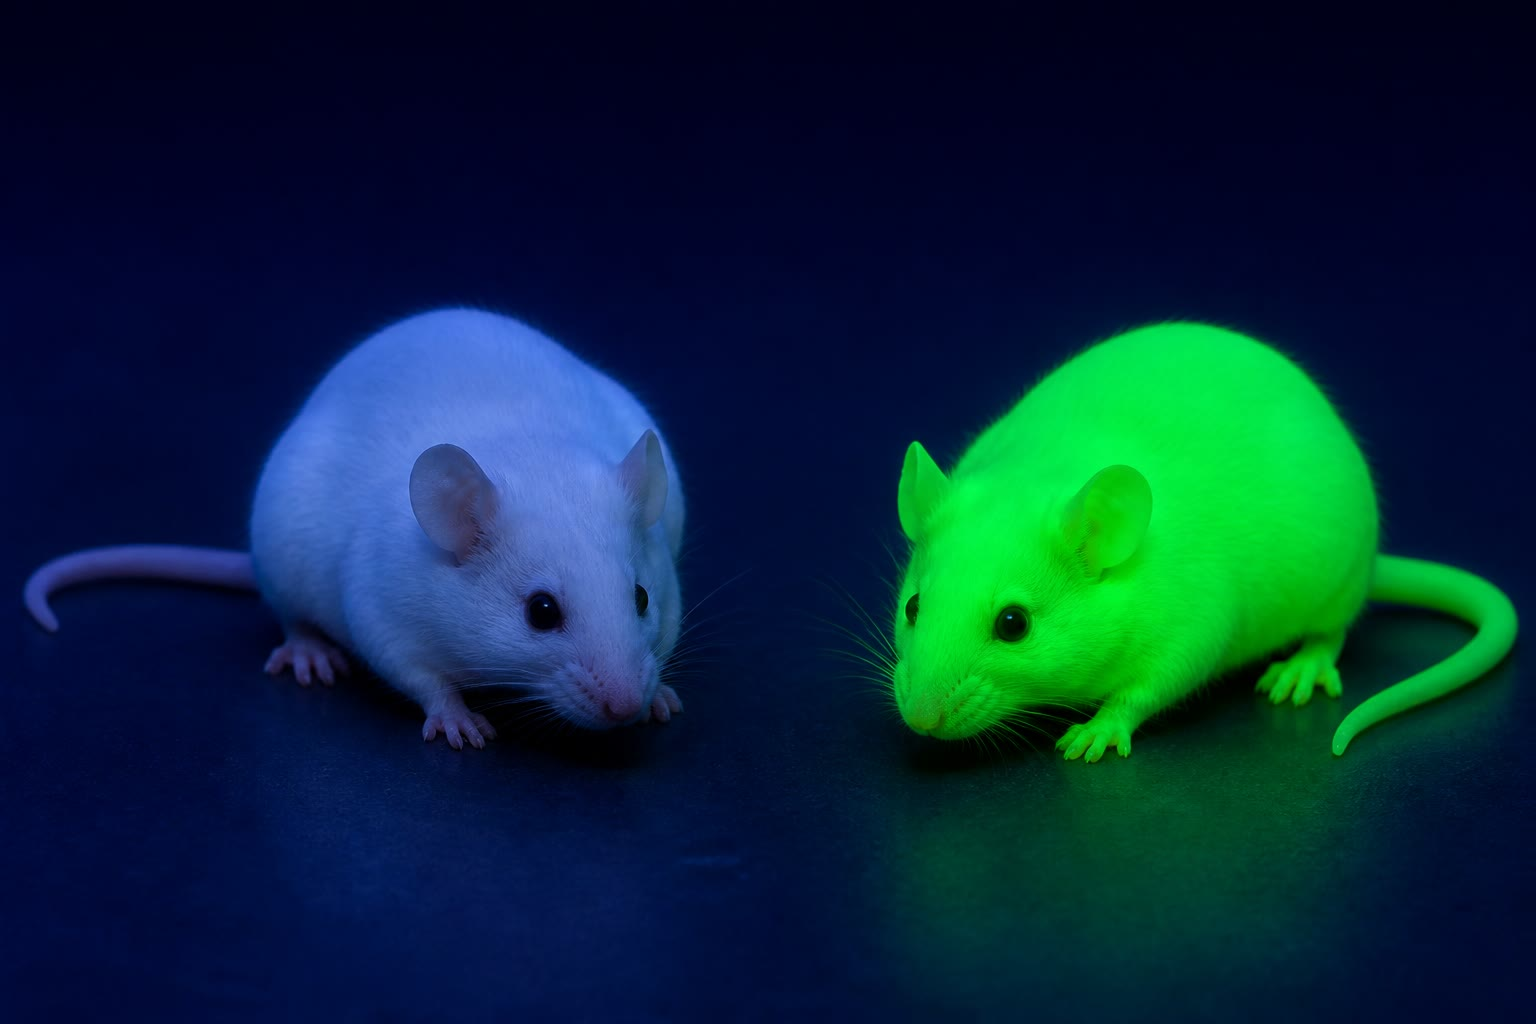
\includegraphics[width=0.62\linewidth]{images/book2/ai/g10-dna-gfp-mice.jpg}

{\small 在蓝光下，携带水母绿色荧光蛋白\omterm{def:g10:universal-dna:gene}{基因}的小鼠
与一只普通小鼠并排发光。分子相同，读取规则相同：
水母的这条遗传指令在
小鼠体内照常运行。}
\end{omfigure}

\begin{example}[转基因技术的应用]\label{ex:g10:universal-dna:uses}
利用细菌生产人胰岛素和生长激素；将抗虫\omterm{def:g10:universal-dna:gene}{基因}
导入玉米或棉花；使水稻携带合成维生素 A 前体的\omterm{def:g10:universal-dna:gene}{基因}；
将 GFP \omterm{def:g10:universal-dna:gene}{基因}连接到另一\omterm{def:g10:universal-dna:gene}{基因}上，
使该\omterm{def:g10:universal-dna:gene}{基因}活跃的\omterm{def:g10:cells-common-unit:cell}{细胞}在显微镜下发光——
最后一种用途作为研究工具，是其中最常见的。
每种用途都引出各自的安全性问题及对环境的影响，
而它们都基于同一事实：
遗传分子具有普遍性。
\end{example}

\begin{remark}[分子水平上的统一性与多样性]\label{rem:g10:universal-dna:unity}
\omterm{def:g10:universal-dna:information}{DNA} 的普遍性是生命统一性在分子层面的体现，
在\cref{ch:g10:chemistry-of-life}中有所说明：
地球上所有生物使用同一种化学体系、同一种信息分子和同一套读取系统，
这正是共同起源所预言的（见\cref{ch:g10:common-ancestry}）。
生命的多样性同样记录在这一分子之中，表现为序列上的差异：
两个\omterm{def:g10:universal-dna:gene}{等位基因}之间相差几个碱基，两个物种之间
\omterm{def:g10:universal-dna:gene}{基因}组相差百分之几，而细菌与人之间
则是整套\omterm{def:g10:universal-dna:information}{遗传信息}的组织方式不同。
\end{remark}

\section{练习}

\begin{exercise}[$\star$]\label{exo:g10:universal-dna:1}
写出\omterm{def:g10:universal-dna:nucleotide}{核苷酸}的三个组成部分和 \omterm{def:g10:universal-dna:information}{DNA} 的四种碱基。
\end{exercise}

\begin{exercise}[$\star$]\label{exo:g10:universal-dna:2}
写出与 \texttt{TACGGATTCA} 互补的链。
\end{exercise}

\begin{exercise}[$\star$]\label{exo:g10:universal-dna:3}
某 \omterm{def:g10:universal-dna:information}{DNA} 样品中鸟嘌呤占 21\%，
求 C、A 和 T 所占的百分比。
\end{exercise}

\begin{exercise}[$\star$]\label{exo:g10:universal-dna:4}
分别用一句话定义\omterm{def:g10:universal-dna:gene}{基因}和\omterm{def:g10:universal-dna:gene}{等位基因}，
并使用“序列”一词。
\end{exercise}

\begin{exercise}[$\star$]\label{exo:g10:universal-dna:5}
什么是转\omterm{def:g10:universal-dna:gene}{基因}生物？举出本章中的两个例子。
\end{exercise}

\begin{exercise}[$\star\star$]\label{exo:g10:universal-dna:6}
一个\omterm{def:g10:universal-dna:gene}{基因}长 1500 个碱基对。其长度为多少纳米，
该\omterm{def:g10:universal-dna:gene}{基因}的螺旋共旋转了多少圈？
\end{exercise}

\begin{exercise}[$\star\star$]\label{exo:g10:universal-dna:7}
计算一个人体\omterm{def:g10:cells-common-unit:cell}{细胞}中 \omterm{def:g10:universal-dna:information}{DNA} 的总长度，已知
每套\omterm{def:g10:universal-dna:information}{染色体}含 $\num{3.2e9}$ 个碱基对，每个\omterm{def:g10:cells-common-unit:cell}{细胞}含两套\omterm{def:g10:universal-dna:information}{染色体}。
将其与\omterm{def:g10:cells-common-unit:organelle}{细胞核}直径 \qty{6}{\micro m} 作比较。
\end{exercise}

\begin{exercise}[$\star\star$]\label{exo:g10:universal-dna:8}
在埃弗里的实验中，为何有必要检验经分解 \omterm{def:g10:universal-dna:information}{DNA} 的酶
处理过的提取物，而不只是纯化的 \omterm{def:g10:universal-dna:information}{DNA}
组分？
\end{exercise}

\begin{exercise}[$\star\star$]\label{exo:g10:universal-dna:9}
解释为什么查加夫的数据排除了这样一种模型：碱基
按规则的重复顺序排列，例如 \texttt{ATGCATGC\dots}
\end{exercise}

\begin{exercise}[$\star\star$]\label{exo:g10:universal-dna:10}
一个\omterm{def:g10:universal-dna:gene}{基因}的两个\omterm{def:g10:universal-dna:gene}{等位基因}在 2000 个碱基中仅相差一个碱基。解释这样的微小差异
如何改变\omterm{def:g10:chemistry-of-life:families}{蛋白质}，以及为何它也可能
不产生任何改变。
\end{exercise}

\begin{exercise}[$\star\star$]\label{exo:g10:universal-dna:11}
导入小鼠受精卵的 GFP \omterm{def:g10:universal-dna:gene}{基因}，在该小鼠的
皮肤\omterm{def:g10:cells-common-unit:cell}{细胞}、肝脏\omterm{def:g10:cells-common-unit:cell}{细胞}和精子中均可找到。请运用\omterm{def:g10:cells-common-unit:cell}{细胞}学说
及\cref{prop:g10:universal-dna:explains}，解释其原因。
\end{exercise}

\begin{exercise}[$\star\star\star$]\label{exo:g10:universal-dna:12}
一个细菌的 \omterm{def:g10:universal-dna:information}{DNA} 分子长 $\num{4.6e6}$ 个碱基对。计算
其长度；与\omterm{def:g10:cells-common-unit:cell}{细胞}的 \qty{2}{\micro m} 相比较；然后
解释细菌为何仍能容纳它。
\end{exercise}

\begin{exercise}[$\star\star\star$]\label{exo:g10:universal-dna:13}
一位朋友声称，人的 \omterm{def:g10:universal-dna:information}{DNA} 必定比细菌的 \omterm{def:g10:universal-dna:information}{DNA}
因碱基更多而“更复杂”。比较 $\num{3.2e9}$ 与
$\num{4.6e6}$ 个碱基对，与 $\num{20000}$ 个、4300 个\omterm{def:g10:universal-dna:gene}{基因}，并讨论
额外的 \omterm{def:g10:universal-dna:information}{DNA} 是什么，又不是什么。
\end{exercise}

\begin{exercise}[$\star\star\star$]\label{exo:g10:universal-dna:14}
设想发现一个物种，其遗传物质所用的
分子与密码都不同。它会与本章的哪些命题相矛盾，
以及这对该物种与其他生命的
共同起源意味着什么？
\end{exercise}

\begin{exercise}[$\star\star\star$]\label{exo:g10:universal-dna:15}
细菌生产的人胰岛素取代了从猪
胰腺中提取的胰岛素。列出细菌产物优于后者的两条生物学理由，
以及监管者仍须提出的一个问题。
\end{exercise}

\section{问题：水母基因}

\begin{problem}[{周末问题——一个来自水母的基因进入小鼠之后：
它的长度、它的字母、小鼠为何能够读取它，以及
每个细胞中携带它的两米 DNA}]
\label{pb:g10:universal-dna:1}
水母 \emph{Aequorea victoria} 的绿色荧光蛋白
是由 238 个\omterm{def:g10:chemistry-of-life:families}{氨基酸}组成的链。其\omterm{def:g10:universal-dna:gene}{基因}在实验室中使用时，
为一段 720 个碱基对的 \omterm{def:g10:universal-dna:information}{DNA} 片段。取每个碱基对 \qty{0.34}{nm}，每圈
10 个碱基对，以及小鼠\omterm{def:g10:universal-dna:gene}{基因}组每组\omterm{def:g10:universal-dna:information}{染色体} $\num{2.7e9}$ 个碱基对，
每个\omterm{def:g10:cells-common-unit:cell}{细胞}含两组\omterm{def:g10:universal-dna:information}{染色体}。

\medskip
\noindent\textbf{第一部分——分子。}
\begin{enumerate}
  \item 计算 GFP \omterm{def:g10:universal-dna:gene}{基因}的长度（以纳米计），以及
        它形成的螺旋圈数。
  \item \omterm{def:g10:universal-dna:gene}{基因}的一条链以 \texttt{ATGAGTAAAGGAGAAGAAC} 开始。
        写出互补链。
  \item 在整个\omterm{def:g10:universal-dna:gene}{基因}中，腺嘌呤占碱基的 27\%。求
        其余三种碱基所占的百分比。
  \item 该\omterm{def:g10:universal-dna:gene}{基因}有 720 个碱基对，编码 238 个\omterm{def:g10:chemistry-of-life:families}{氨基酸}。
        计算其比值，并提出这一比值说明每个\omterm{def:g10:chemistry-of-life:families}{氨基酸}由多少个
        碱基决定的假设（
        \cref{ch:g11:gene-expression} 将证实该假设）。
  \item 原则上，720 个碱基能组成多少种不同的序列？
        将答案写成 4 的幂，然后
        用一句话解释为何该序列可称为信息。
\end{enumerate}

\medskip
\noindent\textbf{第二部分——小鼠为何能够读取它。}
\begin{enumerate}[resume]
  \item 说明 \omterm{def:g10:universal-dna:information}{DNA} 的哪一性质使小鼠\omterm{def:g10:cells-common-unit:cell}{细胞}能够
        利用水母\omterm{def:g10:universal-dna:gene}{基因}。
  \item 该\omterm{def:g10:universal-dna:gene}{基因}被导入受精卵，而非导入
        成年小鼠的皮肤中。运用\omterm{def:g10:cells-common-unit:cell}{细胞}学说，解释这一差别
        对\omterm{def:g10:universal-dna:gene}{基因}最终所在位置有何影响。
  \item 成年小鼠的每种组织都会发光。这说明
        其不同\omterm{def:g10:cells-common-unit:cell}{细胞}类型的 \omterm{def:g10:universal-dna:information}{DNA} 含量有何特点？
  \item 发光小鼠与普通小鼠交配。请预测
        后代中是否有发光者，并说明理由。
  \item 对照小鼠注射纯化的 GFP 蛋白，而非该\omterm{def:g10:universal-dna:gene}{基因}：
        它会微弱发光数天，随后停止。
        解释两个实验的差别。
\end{enumerate}

\medskip
\noindent\textbf{第三部分——故事背后的证据。}
\begin{enumerate}[resume]
  \item 在埃弗里的实验中，指出使细菌发生转化的组分，
        以及消除转化的处理。
  \item 说明转化实验为何是
        \omterm{prop:g10:universal-dna:universal}{转基因技术}的一个自然版本。
  \item 查加夫发现，每个物种中均有 A$\,=\,$T 与 G$\,=\,$C，但
        A+T 所占比例在 25\% 至 75\% 之间变化。两个观察结果中，哪一个
        支持碱基配对，哪一个说明序列是
        自由的？
  \item 富兰克林的照片给出螺旋的直径为
        \qty{2}{nm}。解释为何将一大一小的碱基配对
        （A 与 T、G 与 C），而非两个大碱基配对，
        能使螺旋结构规则。
  \item 结构的发现为何立即暗示了
        \omterm{def:g10:universal-dna:information}{DNA} 如何复制？
\end{enumerate}

\medskip
\noindent\textbf{第四部分——\omterm{def:g10:cells-common-unit:organelle}{细胞核}中的两米。}
\begin{enumerate}[resume]
  \item 计算一个小鼠\omterm{def:g10:cells-common-unit:cell}{细胞}中 \omterm{def:g10:universal-dna:information}{DNA} 的总长度。
  \item \omterm{def:g10:cells-common-unit:organelle}{细胞核}直径为 \qty{6}{\micro m}。\omterm{def:g10:universal-dna:information}{DNA} 须通过盘绕缩短多少倍
        才能容纳？
  \item GFP \omterm{def:g10:universal-dna:gene}{基因}占\omterm{def:g10:cells-common-unit:cell}{细胞} \omterm{def:g10:universal-dna:information}{DNA} 的比例是多少？
  \item 小鼠约有 $\num{2e4}$ 个\omterm{def:g10:universal-dna:gene}{基因}，平均每个\omterm{def:g10:universal-dna:gene}{基因}
        含 $\num{3e4}$ 个碱基对（包括非编码部分）。\omterm{def:g10:universal-dna:gene}{基因}占\omterm{def:g10:universal-dna:gene}{基因}组
        的比例是多少？
  \item 用一句话陈述结果：一个小鼠\omterm{def:g10:cells-common-unit:cell}{细胞}携带多少 \omterm{def:g10:universal-dna:information}{DNA}，
        以及 \omterm{def:g10:universal-dna:information}{DNA} 的哪一个单一事实，使其数千个\omterm{def:g10:universal-dna:gene}{基因}中的
        一个水母\omterm{def:g10:universal-dna:gene}{基因}能够被读取？
\end{enumerate}
\end{problem}
